\graphicspath{./anexos}
\subsection{Modelagem}
Com base no escopo apresentado nas seções anteriores a equipe elaborou a modelagem a partir de diagramas \ac{mer} e \ac{der}.

\subsubsection{MER}
O \ac{Modelo Conceitual} exibe detalhes a serem considerados acerca das entidades, atributos e relacionamentos do sistema no momento da projeção do modelo físico, identificando chaves primárias e estrangeiras. Embora o \ac{mer} possa utilizar atributos, o seguinte \ac{mer} não conta com atributos, a fim de proporcionar inicialmente uma visão mais clara do sistema. 
    A \autoref{mer} exibe o \ac{mer}.

\begin{figure}[htb]
    \centering
    \caption{\label{mer}MER}
    \frame{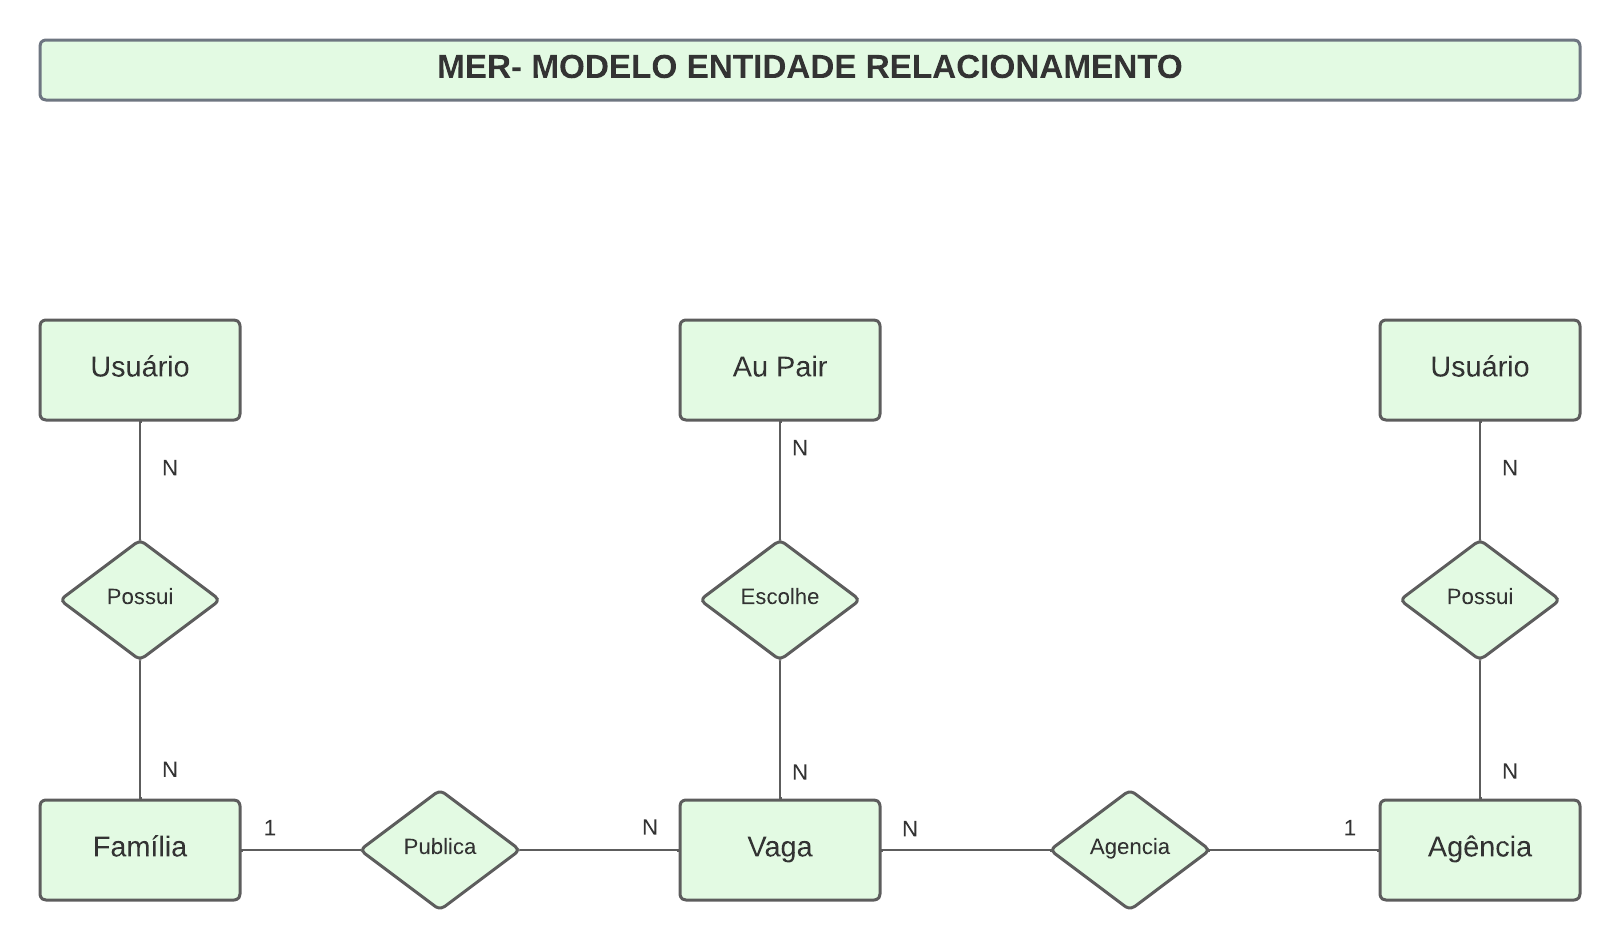
\includegraphics[width=1\textwidth]{anexos/mer.png}}
    \fonte{Autores}
\end{figure}

\subsubsection{DER}
Utilizamos o \ac {der} como representação gráfica do \ac{mer}, que apresenta os atributos de cada entidade citada anteriormente no \ac{mer}. O principal objetivo
do \ac{der} é mostrar as estruturas que irão armazenar os dados, e com isso definir melhor as entidades e os seus atributos.

\begin{figure}[H]
    \centering
    \caption{\label{der}DER}
    \frame{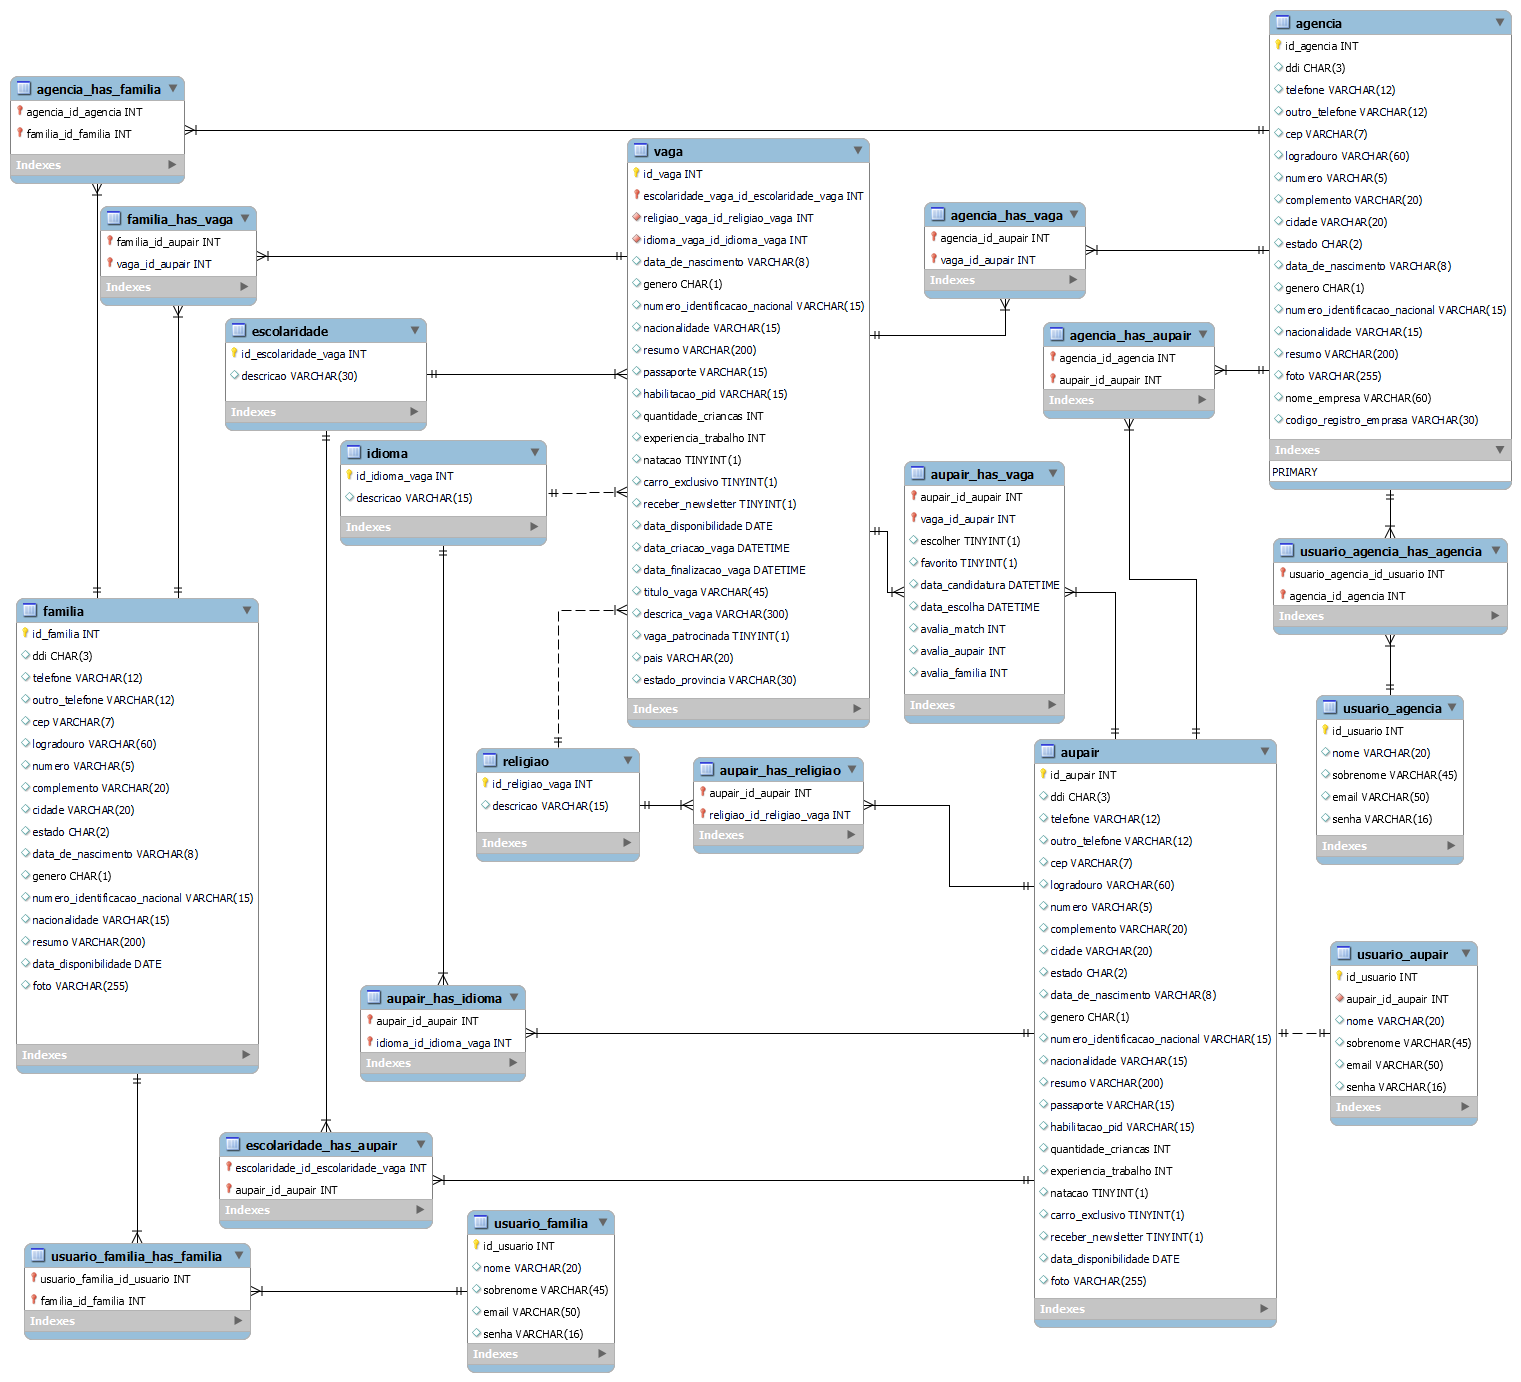
\includegraphics[width=1\textwidth]{anexos/der.png}}
    \fonte{Autores}
\end{figure}

\section{Dicionário de dados}
O dicionário de dados fornece informações adicionais sobre os relacionamentos entre diferentes tabelas de banco de dados além de também ajudar a organizar os dados.

\begin{enumerate}
    \begin{table}[H]
    \caption{Vaga}
    \label{vaga}
    	\centering\footnotesize
        \begin{tabular}{|p{0.40\linewidth} | p{0.04\linewidth} |  p{0.12\linewidth} | p{0.16\linewidth} |}  \hline
        \multicolumn{1}{|c|}{\textbf{Atributos}} &
        \multicolumn{1}{|c|}{\textbf{Chave}} &
        \multicolumn{1}{c|}{\textbf{Descrição}} &
        \multicolumn{1}{c|}{\textbf{Tipo}} \\ \hline
          
        id\_vaga  &  
        PK & 
        Identificador único do registro na tabela de vaga. &
        INT
        \\  \hline
        
        escolaridade\_vaga\_id\_escolaridade\_vaga & 
        FK & 
        Identificador do registro na tabela escolaridade. &
        INT
        \\ \hline
        
       religiao\_vaga\_id\_religiao\_vaga &
       FK &
       Identificador do registro na tabela religiao. &
       INT
       \\ \hline
       
       idioma\_vaga\_id\_idioma\_vaga &
       FK &
       Identificador do registro na tabela idioma. &
       INT
       \\ \hline
       
       data\_de\_nascimento &
       - &
       Data de nascimento. &
       VARCHAR(8)
       \\ \hline
       
       genero &
       - &
       Gênero &
       CHAR(1)
       \\ \hline
       
       numero\_identificacao\_nacional &
       - &
       Número da identidade &
       VARCHAR(15)
       \\ \hline
       
       nacionalidade &
       - &
       Nacionalidade &
       VARCHAR(15)
       \\ \hline
       
       resumo &
       - &
       Resumo &
       VARCHAR(200)
       \\ \hline
       
       passaporte &
       - &
       Passaporte &
       VARCHAR(15)
       \\ \hline
       
       habilitacao\_pid &
       - &
       Permissão internacional para dirigir &
       VARCHAR(15)
       \\ \hline
       
       quantidade\_criancas &
       - &
       Quantidade de crianças &
       INT
       \\ \hline
       
       experiencia\_trabalho &
       - &
       Número de horas de experiência com criança &
       INT
       \\ \hline
       
       natacao &
       - &
       Natação &
       TINYINT(1)
       \\ \hline
       
       carro\_exclusivo &
       - &
       Carro exclusivo para dirigir &
       TINYINT(1)
       \\ \hline
       
       receber\_newsletter &
       - &
       Se deseja receber newsletter &
       TINYINT(1)
       \\ \hline
       
       data\_disponibilidade &
       - &
       Data de disponibilidade &
       DATE
       \\ \hline
       
       data\_criacao\_vaga &
       - &
       Data de criação da vaga &
       DATETIME
       \\ \hline
       
       data\_finalizacao\_vaga &
       - &
       Data de finalização da vaga &
       DATETIME
       \\ \hline
       
       titulo\_vaga &
       - &
       Título da vaga &
       VARCHAR(45)
       \\ \hline
       
       descricao\_vaga &
       - &
       Descrição da vaga &
       VARCHAR(300)
       \\ \hline
       
       vaga\_patrocinada &
       - &
       Se a vaga é pratrocinada &
       TINYINT(1)
       \\ \hline
       
       pais &
       - &
       País &
       VARCHAR(20)
       \\ \hline
       
       estado\_provincia &
       - &
       Estado &
       VARCHAR(30)
       \\ \hline
       
        \end{tabular}
    \fonte{Autores}
    \end{table}
\end{enumerate}

\begin{enumerate}
    \begin{table}[H]
    \caption{regiliao}
    \label{regiliao}
    	\centering\footnotesize
        \begin{tabular}{|p{0.40\linewidth} | p{0.04\linewidth} |  p{0.12\linewidth} | p{0.16\linewidth} |}  \hline
        \multicolumn{1}{|c|}{\textbf{Atributos}} &
        \multicolumn{1}{|c|}{\textbf{Chave}} &
        \multicolumn{1}{c|}{\textbf{Descrição}} &
        \multicolumn{1}{c|}{\textbf{Tipo}} \\ \hline
          
        id\_religiao  &  
        PK & 
        Identificador único do registro na tabela de religiao. &
        INT
        \\  \hline
        
        descricao & 
        - & 
        Descrição &
        VARCHAR(15)
        \\ \hline
       
        \end{tabular}
    \fonte{Autores}
    \end{table}
\end{enumerate}

\begin{enumerate}
    \begin{table}[H]
    \caption{escolaridade}
    \label{escolaridade}
    	\centering\footnotesize
        \begin{tabular}{|p{0.40\linewidth} | p{0.04\linewidth} |  p{0.12\linewidth} | p{0.16\linewidth} |}  \hline
        \multicolumn{1}{|c|}{\textbf{Atributos}} &
        \multicolumn{1}{|c|}{\textbf{Chave}} &
        \multicolumn{1}{c|}{\textbf{Descrição}} &
        \multicolumn{1}{c|}{\textbf{Tipo}} \\ \hline
          
        id\_escolaridade  &  
        PK & 
        Identificador único do registro na tabela de escolaridade. &
        INT
        \\  \hline
        
        descricao & 
        - & 
        Descrição &
        VARCHAR(15)
        \\ \hline
       
        \end{tabular}
    \fonte{Autores}
    \end{table}
\end{enumerate}

\begin{enumerate}
    \begin{table}[H]
    \caption{idioma}
    \label{idioma}
    	\centering\footnotesize
        \begin{tabular}{|p{0.40\linewidth} | p{0.04\linewidth} |  p{0.12\linewidth} | p{0.16\linewidth} |}  \hline
        \multicolumn{1}{|c|}{\textbf{Atributos}} &
        \multicolumn{1}{|c|}{\textbf{Chave}} &
        \multicolumn{1}{c|}{\textbf{Descrição}} &
        \multicolumn{1}{c|}{\textbf{Tipo}} \\ \hline
          
        id\_idioma  &  
        PK & 
        Identificador único do registro na tabela de idioma. &
        INT
        \\  \hline
        
        descricao & 
        - & 
        Descrição &
        VARCHAR(30)
        \\ \hline
       
        \end{tabular}
    \fonte{Autores}
    \end{table}
\end{enumerate}

\begin{enumerate}
    \begin{table}[H]
    \caption{familia\_has\_vaga}
    \label{idioma}
    	\centering\footnotesize
        \begin{tabular}{|p{0.40\linewidth} | p{0.04\linewidth} |  p{0.12\linewidth} | p{0.16\linewidth} |}  \hline
        \multicolumn{1}{|c|}{\textbf{Atributos}} &
        \multicolumn{1}{|c|}{\textbf{Chave}} &
        \multicolumn{1}{c|}{\textbf{Descrição}} &
        \multicolumn{1}{c|}{\textbf{Tipo}} \\ \hline
          
        familia\_id\_vaga  &  
        FK & 
        Identificador único do registro na tabela de vaga &
        INT
        \\  \hline
        
        vaga\_id\_aupair  &  
        FK & 
        Identificador único do registro na tabela de au pair &
        INT
        \\  \hline
       
        \end{tabular}
    \fonte{Autores}
    \end{table}
\end{enumerate}

\begin{enumerate}
    \begin{table}[H]
    \caption{aupair\_has\_vaga}
    \label{idioma}
    	\centering\footnotesize
        \begin{tabular}{|p{0.40\linewidth} | p{0.04\linewidth} |  p{0.12\linewidth} | p{0.16\linewidth} |}  \hline
        \multicolumn{1}{|c|}{\textbf{Atributos}} &
        \multicolumn{1}{|c|}{\textbf{Chave}} &
        \multicolumn{1}{c|}{\textbf{Descrição}} &
        \multicolumn{1}{c|}{\textbf{Tipo}} \\ \hline
          
        aupair\_id\_aupair  &  
        FK & 
        Identificador único do registro na tabela de au pair &
        INT
        \\  \hline
        
        vaga\_id\_aupair  &  
        FK & 
        Identificador único do registro na tabela de au pair &
        INT
        \\  \hline
        
        escolher  &  
        - & 
        Confirmação de candidato selecionado para vaga &
        TINYINT(1)
        \\  \hline
        
        favorito  &  
        - & 
        Vagas favoritas &
        TINYINT(1)
        \\  \hline
        
        data\_candidatura  &  
        - & 
        Data da candidatura &
        DATETIME
        \\  \hline
        
        data\_escolha  &  
        - & 
        Data da escolha da vaga &
        DATETIME
        \\  \hline
        
        avalia\_match  &  
        - & 
        Avaliar o match &
        INT
        \\  \hline
        
        avalia\_aupair  &  
        - & 
        Avaliar au pair &
        INT
        \\  \hline
        
        avalia\_familia  &  
        - & 
        Avaliar familia &
        INT
        \\  \hline
       
       
        \end{tabular}
    \fonte{Autores}
    \end{table}
\end{enumerate}

\begin{enumerate}
    \begin{table}[H]
    \caption{aupair\_has\_religiao}
    \label{idioma}
    	\centering\footnotesize
        \begin{tabular}{|p{0.40\linewidth} | p{0.04\linewidth} |  p{0.12\linewidth} | p{0.16\linewidth} |}  \hline
        \multicolumn{1}{|c|}{\textbf{Atributos}} &
        \multicolumn{1}{|c|}{\textbf{Chave}} &
        \multicolumn{1}{c|}{\textbf{Descrição}} &
        \multicolumn{1}{c|}{\textbf{Tipo}} \\ \hline
          
        aupair\_id\_aupair  &  
        FK & 
        Identificador único do registro na tabela de aupair &
        INT
        \\  \hline
        
        religiao\_id\_religiao\_vaga  &  
        FK & 
        Identificador único do registro na tabela de vaga &
        INT
        \\  \hline
       
        \end{tabular}
    \fonte{Autores}
    \end{table}
\end{enumerate}

\begin{enumerate}
    \begin{table}[H]
    \caption{aupair\_has\_idioma}
    \label{idioma}
    	\centering\footnotesize
        \begin{tabular}{|p{0.40\linewidth} | p{0.04\linewidth} |  p{0.12\linewidth} | p{0.16\linewidth} |}  \hline
        \multicolumn{1}{|c|}{\textbf{Atributos}} &
        \multicolumn{1}{|c|}{\textbf{Chave}} &
        \multicolumn{1}{c|}{\textbf{Descrição}} &
        \multicolumn{1}{c|}{\textbf{Tipo}} \\ \hline
          
        aupair\_id\_aupair  &  
        FK & 
        Identificador único do registro na tabela de aupair &
        INT
        \\  \hline
        
        idioma\_id\_idioma\_vaga  &  
        FK & 
        Identificador único do registro na tabela de vaga &
        INT
        \\  \hline
       
        \end{tabular}
    \fonte{Autores}
    \end{table}
\end{enumerate}

\begin{enumerate}
    \begin{table}[H]
    \caption{familia}
    \label{idioma}
    	\centering\footnotesize
        \begin{tabular}{|p{0.40\linewidth} | p{0.04\linewidth} |  p{0.12\linewidth} | p{0.16\linewidth} |}  \hline
        \multicolumn{1}{|c|}{\textbf{Atributos}} &
        \multicolumn{1}{|c|}{\textbf{Chave}} &
        \multicolumn{1}{c|}{\textbf{Descrição}} &
        \multicolumn{1}{c|}{\textbf{Tipo}} \\ \hline
          
        id\_familia  &  
        PK & 
        Identificador único do registro na tabela de familia &
        INT
        \\  \hline
        
        ddi  &  
        - & 
        Discagem direta internacional &
        CHAR(3)
        \\  \hline
        
        telefone  &  
        - & 
        Telefone &
        VARCHAR(12)
        \\  \hline
        
        outro\_telefone  &  
        - & 
        Telefone &
        VARCHAR(12)
        \\  \hline
        
        cep  &  
        - & 
        CEP &
        VARCHAR(7)
        \\  \hline
        
        logradouro  &  
        - & 
        Logradouro &
        VARCHAR(60)
        \\  \hline
        
        numero  &  
        - & 
        Número &
        VARCHAR(5)
        \\  \hline
        
        complemento  &  
        - & 
        Complemento &
        VARCHAR(20)
        \\  \hline
        
        cidade  &  
        - & 
        Cidade &
        VARCHAR(20)
        \\  \hline
        
        estado  &  
        - & 
        Estado &
        CHAR(2)
        \\  \hline
        
        data\_de\_nascimento  &  
        - & 
        Data de nascimento &
        VARCHAR(8)
        \\  \hline
        
        genero  &  
        - & 
        Gênero &
        CHAR(1)
        \\  \hline
        
        numero\_identificacao\_nacional  &  
        - & 
        Número da identificação &
        VARCHAR(15)
        \\  \hline
        
        nacionalidade  &  
        - & 
        Nacionalidade &
        VARCHAR(15)
        \\  \hline
        
        resumo  &  
        - & 
        Resumo &
        VARCHAR(200)
        \\  \hline
        
        data\_disponibilidade  &  
        - & 
        Data de disponibilidade &
        DATE
        \\  \hline
        
        foto  &  
        - & 
        Foto &
        VARCHAR(255)
        \\  \hline
       
        \end{tabular}
    \fonte{Autores}
    \end{table}
\end{enumerate}

\begin{enumerate}
    \begin{table}[H]
    \caption{usuario\_familia}
    \label{idioma}
    	\centering\footnotesize
        \begin{tabular}{|p{0.40\linewidth} | p{0.04\linewidth} |  p{0.12\linewidth} | p{0.16\linewidth} |}  \hline
        \multicolumn{1}{|c|}{\textbf{Atributos}} &
        \multicolumn{1}{|c|}{\textbf{Chave}} &
        \multicolumn{1}{c|}{\textbf{Descrição}} &
        \multicolumn{1}{c|}{\textbf{Tipo}} \\ \hline
          
        id\_familia  &  
        PK & 
        Identificador único do registro na tabela de usuario\_familia &
        INT
        \\  \hline
        
        nome  &  
        - & 
        Nome &
        VARCHAR(20)
        \\  \hline
        
        sobrenome  &  
        - & 
        Sobrenome &
        VARCHAR(45)
        \\  \hline
        
        email  &  
        - & 
        Email &
        VARCHAR(50)
        \\  \hline
        
        senha  &  
        - & 
        Senha &
        VARCHAR(16)
        \\  \hline
       
        \end{tabular}
    \fonte{Autores}
    \end{table}
\end{enumerate}


\begin{enumerate}
    \begin{table}[H]
    \caption{agencia\_has\_familia}
    \label{idioma}
    	\centering\footnotesize
        \begin{tabular}{|p{0.40\linewidth} | p{0.04\linewidth} |  p{0.12\linewidth} | p{0.16\linewidth} |}  \hline
        \multicolumn{1}{|c|}{\textbf{Atributos}} &
        \multicolumn{1}{|c|}{\textbf{Chave}} &
        \multicolumn{1}{c|}{\textbf{Descrição}} &
        \multicolumn{1}{c|}{\textbf{Tipo}} \\ \hline
          
        agencia\_id\_agencia  &  
        FK & 
        Identificador único do registro na tabela de agencia &
        INT
        \\  \hline
        
        familia\_id\_familia  &  
        FK & 
        Identificador único do registro na tabela de familia &
        INT
        \\  \hline
       
        \end{tabular}
    \fonte{Autores}
    \end{table}
\end{enumerate}


\begin{enumerate}
    \begin{table}[H]
    \caption{agencia\_has\_vaga}
    \label{idioma}
    	\centering\footnotesize
        \begin{tabular}{|p{0.40\linewidth} | p{0.04\linewidth} |  p{0.12\linewidth} | p{0.16\linewidth} |}  \hline
        \multicolumn{1}{|c|}{\textbf{Atributos}} &
        \multicolumn{1}{|c|}{\textbf{Chave}} &
        \multicolumn{1}{c|}{\textbf{Descrição}} &
        \multicolumn{1}{c|}{\textbf{Tipo}} \\ \hline
          
        agencia\_id\_aupair  &  
        FK & 
        Identificador único do registro na tabela de au pair &
        INT
        \\  \hline
        
        vaga\_id\_aupair  &  
        FK & 
        Identificador único do registro na tabela de au pair &
        INT
        \\  \hline
       
        \end{tabular}
    \fonte{Autores}
    \end{table}
\end{enumerate}

\begin{enumerate}
    \begin{table}[H]
    \caption{agencia}
    \label{idioma}
    	\centering\footnotesize
        \begin{tabular}{|p{0.40\linewidth} | p{0.04\linewidth} |  p{0.12\linewidth} | p{0.16\linewidth} |}  \hline
        \multicolumn{1}{|c|}{\textbf{Atributos}} &
        \multicolumn{1}{|c|}{\textbf{Chave}} &
        \multicolumn{1}{c|}{\textbf{Descrição}} &
        \multicolumn{1}{c|}{\textbf{Tipo}} \\ \hline
          
        id\_agencia &  
        PK & 
        Identificador único do registro na tabela de agencia &
        INT
        \\  \hline
        
        ddi  &  
        - & 
        Discagem direta internacional &
        CHAR(3)
        \\  \hline
        
        telefone  &  
        - & 
        Telefone &
        VARCHAR(12)
        \\  \hline
        
        outro\_telefone  &  
        - & 
        Telefone &
        VARCHAR(12)
        \\  \hline
        
        cep  &  
        - & 
        CEP &
        VARCHAR(7)
        \\  \hline
        
        logradouro  &  
        - & 
        Logradouro &
        VARCHAR(60)
        \\  \hline
        
        numero  &  
        - & 
        Número &
        VARCHAR(5)
        \\  \hline
        
        complemento  &  
        - & 
        Complemento &
        VARCHAR(20)
        \\  \hline
        
        cidade  &  
        - & 
        Cidade &
        VARCHAR(20)
        \\  \hline
        
        estado  &  
        - & 
        Estado &
        CHAR(2)
        \\  \hline
        
        data\_de\_nascimento  &  
        - & 
        Data de nascimento &
        VARCHAR(8)
        \\  \hline
        
        genero  &  
        - & 
        Gênero &
        CHAR(1)
        \\  \hline
        
        numero\_identificacao\_nacional  &  
        - & 
        Número da identificação &
        VARCHAR(15)
        \\  \hline
        
        nacionalidade  &  
        - & 
        Nacionalidade &
        VARCHAR(15)
        \\  \hline
        
        resumo  &  
        - & 
        Resumo &
        VARCHAR(200)
        \\  \hline
        
        foto  &  
        - & 
        Foto &
        VARCHAR(255)
        \\  \hline
        
        nome\_empresa  &  
        - & 
        Nome da empresa &
        VARCHAR(60)
        \\  \hline
        
        codigo\_registro\_empresa  &  
        - & 
        Código de registro da empresa &
        VARCHAR(30)
        \\  \hline
       
        \end{tabular}
    \fonte{Autores}
    \end{table}
\end{enumerate}

\begin{enumerate}
    \begin{table}[H]
    \caption{agencia\_has\_aupair}
    \label{idioma}
    	\centering\footnotesize
        \begin{tabular}{|p{0.40\linewidth} | p{0.04\linewidth} |  p{0.12\linewidth} | p{0.16\linewidth} |}  \hline
        \multicolumn{1}{|c|}{\textbf{Atributos}} &
        \multicolumn{1}{|c|}{\textbf{Chave}} &
        \multicolumn{1}{c|}{\textbf{Descrição}} &
        \multicolumn{1}{c|}{\textbf{Tipo}} \\ \hline
          
        agencia\_id\_agencia  &  
        FK & 
        Identificador único do registro na tabela de agencia &
        INT
        \\  \hline
        
        aupair\_id\_aupair &  
        FK & 
        Identificador único do registro na tabela de au pair &
        INT
        \\  \hline
       
        \end{tabular}
    \fonte{Autores}
    \end{table}
\end{enumerate}

\begin{enumerate}
    \begin{table}[H]
    \caption{usuario\_agencia}
    \label{idioma}
    	\centering\footnotesize
        \begin{tabular}{|p{0.40\linewidth} | p{0.04\linewidth} |  p{0.12\linewidth} | p{0.16\linewidth} |}  \hline
        \multicolumn{1}{|c|}{\textbf{Atributos}} &
        \multicolumn{1}{|c|}{\textbf{Chave}} &
        \multicolumn{1}{c|}{\textbf{Descrição}} &
        \multicolumn{1}{c|}{\textbf{Tipo}} \\ \hline
          
        id\_agencia &  
        PK & 
        Identificador único do registro na tabela de usuario\_agencia &
        INT
        \\  \hline
        
        nome  &  
        - & 
        Nome &
        VARCHAR(20)
        \\  \hline
        
        sobrenome  &  
        - & 
        Sobrenome &
        VARCHAR(45)
        \\  \hline
        
        email  &  
        - & 
        Email &
        VARCHAR(50)
        \\  \hline
        
        senha  &  
        - & 
        Senha &
        VARCHAR(16)
        \\  \hline
       
        \end{tabular}
    \fonte{Autores}
    \end{table}
\end{enumerate}

\begin{enumerate}
    \begin{table}[H]
    \caption{agencia\_has\_agencia}
    \label{idioma}
    	\centering\footnotesize
        \begin{tabular}{|p{0.40\linewidth} | p{0.04\linewidth} |  p{0.12\linewidth} | p{0.16\linewidth} |}  \hline
        \multicolumn{1}{|c|}{\textbf{Atributos}} &
        \multicolumn{1}{|c|}{\textbf{Chave}} &
        \multicolumn{1}{c|}{\textbf{Descrição}} &
        \multicolumn{1}{c|}{\textbf{Tipo}} \\ \hline
          
        usuario\_agencia\_id\_usuario  &  
        FK & 
        Identificador único do registro na tabela de usuario\_agencia &
        INT
        \\  \hline
        
        agencia\_id\_agencia &  
        FK & 
        Identificador único do registro na tabela de agencia &
        INT
        \\  \hline
       
        \end{tabular}
    \fonte{Autores}
    \end{table}
\end{enumerate}

\begin{enumerate}
    \begin{table}[H]
    \caption{usuario\_aupair}
    \label{idioma}
    	\centering\footnotesize
        \begin{tabular}{|p{0.40\linewidth} | p{0.04\linewidth} |  p{0.12\linewidth} | p{0.16\linewidth} |}  \hline
        \multicolumn{1}{|c|}{\textbf{Atributos}} &
        \multicolumn{1}{|c|}{\textbf{Chave}} &
        \multicolumn{1}{c|}{\textbf{Descrição}} &
        \multicolumn{1}{c|}{\textbf{Tipo}} \\ \hline
          
        id\_usuario &  
        PK & 
        Identificador único do registro na tabela de usuario\_aupair &
        INT
        \\  \hline
        
        aupair\_id\_aupair  &  
        FK & 
        Identificador único do registro na tabela de aupair &
        INT
        \\  \hline
        
        nome  &  
        - & 
        Nome &
        VARCHAR(20)
        \\  \hline
        
        sobrenome  &  
        - & 
        Sobrenome &
        VARCHAR(45)
        \\  \hline
        
        email  &  
        - & 
        Email &
        VARCHAR(50)
        \\  \hline
        
        senha  &  
        - & 
        Senha &
        VARCHAR(16)
        \\  \hline
       
        \end{tabular}
    \fonte{Autores}
    \end{table}
\end{enumerate}

\begin{enumerate}
    \begin{table}[H]
    \caption{aupair}
    \label{idioma}
    	\centering\footnotesize
        \begin{tabular}{|p{0.40\linewidth} | p{0.04\linewidth} |  p{0.12\linewidth} | p{0.16\linewidth} |}  \hline
        \multicolumn{1}{|c|}{\textbf{Atributos}} &
        \multicolumn{1}{|c|}{\textbf{Chave}} &
        \multicolumn{1}{c|}{\textbf{Descrição}} &
        \multicolumn{1}{c|}{\textbf{Tipo}} \\ \hline
          
        id\_aupair  &  
        PK & 
        Identificador único do registro na tabela de aupair &
        INT
        \\  \hline
        
        ddi  &  
        - & 
        Discagem direta internacional &
        CHAR(3)
        \\  \hline
        
        telefone  &  
        - & 
        Telefone &
        VARCHAR(12)
        \\  \hline
        
        outro\_telefone  &  
        - & 
        Telefone &
        VARCHAR(12)
        \\  \hline
        
        cep  &  
        - & 
        CEP &
        VARCHAR(7)
        \\  \hline
        
        logradouro  &  
        - & 
        Logradouro &
        VARCHAR(60)
        \\  \hline
        
        numero  &  
        - & 
        Número &
        VARCHAR(5)
        \\  \hline
        
        complemento  &  
        - & 
        Complemento &
        VARCHAR(20)
        \\  \hline
        
        cidade  &  
        - & 
        Cidade &
        VARCHAR(20)
        \\  \hline
        
        estado  &  
        - & 
        Estado &
        CHAR(2)
        \\  \hline
        
        data\_de\_nascimento  &  
        - & 
        Data de nascimento &
        VARCHAR(8)
        \\  \hline
        
        genero  &  
        - & 
        Gênero &
        CHAR(1)
        \\  \hline
        
        numero\_identificacao\_nacional  &  
        - & 
        Número da identificação &
        VARCHAR(15)
        \\  \hline
        
        nacionalidade  &  
        - & 
        Nacionalidade &
        VARCHAR(15)
        \\  \hline
        
        resumo  &  
        - & 
        Resumo &
        VARCHAR(200)
        \\  \hline
        
        data\_disponibilidade  &  
        - & 
        Data de disponibilidade &
        DATE
        \\  \hline
        
        foto  &  
        - & 
        Foto &
        VARCHAR(255)
        \\  \hline
       
        \end{tabular}
    \fonte{Autores}
    \end{table}
\end{enumerate}

\begin{enumerate}
    \begin{table}[H]
    \caption{escolaridade\_has\_aupair}
    \label{idioma}
    	\centering\footnotesize
        \begin{tabular}{|p{0.40\linewidth} | p{0.04\linewidth} |  p{0.12\linewidth} | p{0.16\linewidth} |}  \hline
        \multicolumn{1}{|c|}{\textbf{Atributos}} &
        \multicolumn{1}{|c|}{\textbf{Chave}} &
        \multicolumn{1}{c|}{\textbf{Descrição}} &
        \multicolumn{1}{c|}{\textbf{Tipo}} \\ \hline
          
        escolaridade\_id\_escolaridade\_vaga  &  
        FK & 
        Identificador único do registro na tabela de vaga &
        INT
        \\  \hline
        
        aupair\_id\_aupair &  
        FK & 
        Identificador único do registro na tabela de aupair &
        INT
        \\  \hline
       
        \end{tabular}
    \fonte{Autores}
    \end{table}
\end{enumerate}



